% Szablon: mgr inż. Dawid Kotlarski, 06.10.2024.
% Dokumentacja projektowa aktualnej wersji programu.
\documentclass[12pt,twoside,a4paper]{article}

% Pakiety potrzebne do bieżącej dokumentacji.
\usepackage{cmap}
\usepackage[T1]{fontenc}
\usepackage[utf8]{inputenc}
\usepackage{lmodern}
\IfFileExists{polish.ldf}{%
  \usepackage[polish]{babel}%
}{%
  \usepackage{babel}%
  \babelprovide[main,import]{polish}%
}
\usepackage{amsmath,amssymb}
\usepackage{microtype}
\usepackage[final]{graphicx}
\usepackage[a4paper,left=3.5cm,right=2.5cm,top=2.5cm,bottom=2.5cm]{geometry}
\usepackage{xcolor}
\usepackage{strona_tytulowa}
\usepackage[sf,bf]{titlesec}
\usepackage{tocloft}
\usepackage{array,tabularx}
\usepackage{float}
\usepackage[section]{placeins}
\usepackage{needspace}
\usepackage{listings}
\usepackage[format=hang,labelsep=period,labelfont={bf,small},textfont=small]{caption}
\usepackage{tikz}
\usetikzlibrary{positioning,arrows.meta,shapes.multipart}
\usepackage{fancyhdr}
\usepackage[
  unicode=true,colorlinks=true,urlcolor=blue,linkcolor=black,citecolor=black,
  bookmarksopen=true,bookmarksnumbered=true,pdfstartview=FitH
]{hyperref}

\definecolor{codegreen}{rgb}{0,0.45,0}
\definecolor{codegray}{rgb}{0.45,0.45,0.45}
\definecolor{codepurple}{rgb}{0.58,0,0.72}
\definecolor{backcolour}{rgb}{0.95,0.95,0.92}
\lstdefinestyle{mystyle}{
  language=C++,
  backgroundcolor=\color{backcolour},
  commentstyle=\color{codegreen},
  keywordstyle=\color{blue},
  numberstyle=\tiny\color{codegray},
  stringstyle=\color{codepurple},
  basicstyle=\ttfamily\footnotesize\bezligaturkodu,
  breaklines=true,breakatwhitespace=false,
  captionpos=b,keepspaces=true,numbers=left,numbersep=6pt,
  showspaces=false,showstringspaces=false,showtabs=false,tabsize=4,
  columns=fullflexible,
  xleftmargin=1.5em,framexleftmargin=0.4em,
  aboveskip=7pt,belowskip=5pt,
  literate=
    {ą}{{\k{a}}}1 {ć}{{\'c}}1 {ę}{{\k{e}}}1 {ł}{{\l}}1
    {ń}{{\'n}}1 {ó}{{\'o}}1 {ś}{{\'s}}1 {ź}{{\'z}}1 {ż}{{\.z}}1
    {Ą}{{\k{A}}}1 {Ć}{{\'C}}1 {Ę}{{\k{E}}}1 {Ł}{{\L}}1
    {Ń}{{\'N}}1 {Ó}{{\'O}}1 {Ś}{{\'S}}1 {Ź}{{\'Z}}1 {Ż}{{\.Z}}1
}
\lstdefinestyle{terminal}{
  style=mystyle,language={},numbers=none,frame=single,
  backgroundcolor=\color{white},xleftmargin=0pt,framexleftmargin=0pt,
  basicstyle=\ttfamily\footnotesize\bezligaturkodu
}
\lstdefinestyle{konfiguracja}{style=mystyle,language={}}
\lstset{style=mystyle}

% Numeracja i wygląd zgodne z układem przekazanego szablonu.
\makeatletter
\def\numberline#1{\hb@xt@\@tempdima{#1.\hfil}}
\renewcommand*\@seccntformat[1]{\csname the#1\endcsname.\enspace}
\@addtoreset{equation}{section}
\renewcommand{\theequation}{\thesection.\arabic{equation}}
\@addtoreset{figure}{section}
\renewcommand{\thefigure}{\thesection.\arabic{figure}}
\@addtoreset{table}{section}
\renewcommand{\thetable}{\thesection.\arabic{table}}
\makeatother

\newenvironment{tabela}[3]{%
  \begin{table}[H]\centering\caption[#1]{#2}\medskip#3%
}{\end{table}}

\newcommand{\bezligaturkodu}{\ifdefined\pdfnoligatures\pdfnoligatures\font\fi}
\newcommand{\kod}[1]{\texttt{\bezligaturkodu\detokenize{#1}}}
\newcolumntype{L}[1]{>{\raggedright\arraybackslash}p{#1}}
\newcolumntype{Y}{>{\raggedright\arraybackslash}X}

% Listing pozostaje przy swoim opisie i nie jest dzielony pomiędzy strony.
\newcommand{\listingpliku}[2][]{%
  \par\smallskip\noindent
  \begin{minipage}{\linewidth}
    \lstinputlisting[#1]{#2}
  \end{minipage}
  \par\smallskip
}

\frenchspacing
\setlength{\parindent}{0.6cm}
\setlength{\parskip}{3pt}
\linespread{1.3}
\raggedbottom
\setcounter{tocdepth}{2}
\setcounter{secnumdepth}{3}
\renewcommand{\arraystretch}{1.18}
\captionsetup[table]{position=top,skip=6pt}
\captionsetup[figure]{skip=7pt}
\setlength{\emergencystretch}{2em}

\renewcommand{\cfttoctitlefont}{\Large\bfseries\sffamily}
\renewcommand{\cftloftitlefont}{\Large\bfseries\sffamily}
\renewcommand{\cftlottitlefont}{\Large\bfseries\sffamily}
\renewcommand{\cftsecfont}{\bfseries\sffamily}
\renewcommand{\cftsubsecfont}{\sffamily}

\pagestyle{fancy}
\fancyhf{}
\fancyhead[C]{\footnotesize\textit{AKADEMIA NAUK STOSOWANYCH W NOWYM SĄCZU}}
\fancyfoot[C]{%
  \scriptsize DOKUMENTACJA PROJEKTU - ZAAWANSOWANE PROGRAMOWANIE\\
  \normalsize\sffamily\thepage
}
\setlength{\headheight}{20pt}
\setlength{\footskip}{35pt}
\renewcommand{\headrulewidth}{0.4pt}
\renewcommand{\footrulewidth}{0.4pt}
\makeatletter
\let\ps@plain\ps@fancy
\makeatother


% Dane strony tytułowej można zmienić w poniższych poleceniach.
\title{Algorytm drzewa BST\\z zastosowaniem GitHub}
\author{Jakub Pyrdoł}
\authorI{Tymoteusz Zaczyk}
\authorII{Dawid Plewa}
\uczelnia{AKADEMIA NAUK STOSOWANYCH\\W NOWYM SĄCZU}
\instytut{Wydział Nauk Inżynieryjnych}
\kierunek{Katedra Informatyki}
\praca{DOKUMENTACJA PROJEKTOWA}
\przedmiot{ZAAWANSOWANE PROGRAMOWANIE}
\prowadzacy{mgr inż. Dawid Kotlarski}
\rok{2026}

\hypersetup{
  pdftitle={Algorytm drzewa BST z zastosowaniem GitHub},
  pdfauthor={Jakub Pyrdoł, Tymoteusz Zaczyk, Dawid Plewa},
  pdfsubject={Dokumentacja bieżącej implementacji drzewa BST}
}

\begin{document}
\renewcommand{\figurename}{Rys.}
\renewcommand{\tablename}{Tab.}
\renewcommand{\refname}{Literatura}
\renewcommand{\lstlistingname}{Listing}
\renewcommand{\lstlistlistingname}{Spis listingów}

\thispagestyle{empty}
\stronatytulowa
\pagestyle{fancy}

\begingroup
\linespread{1}\selectfont
\setlength{\cftbeforesecskip}{5pt}
\setlength{\cftbeforesubsecskip}{1pt}
\setlength{\cftparskip}{0pt}
\tableofcontents
\endgroup

\clearpage
\section{Ogólne określenie wymagań}

Celem projektu jest przygotowanie binarnego drzewa poszukiwań
(BST, ang.~\emph{Binary Search Tree}) przechowującego liczby całkowite.
Program ma przedstawiać sposób organizowania danych w strukturze
drzewiastej oraz umożliwiać dodawanie i usuwanie elementów
z zachowaniem określonego porządku. Projekt obejmuje również
wykorzystanie systemu kontroli wersji Git oraz platformy GitHub
do przechowywania kodu i zapisywania kolejnych etapów jego rozwoju.

Drzewo składa się z węzłów połączonych relacjami rodzic--dziecko.
Węzeł rozpoczynający strukturę nazywany jest korzeniem.
Każdy węzeł drzewa binarnego może mieć najwyżej dwoje dzieci:
lewe i prawe. Węzeł bez dzieci jest liściem, natomiast węzły
znajdujące się poniżej danego elementu tworzą jego poddrzewa.
Taki sposób organizacji danych pozwala opisywać zależności
pomiędzy elementami bez ograniczania ich do jednej kolejności liniowej.

W drzewie BST obowiązuje dodatkowa reguła porządku.
Wszystkie wartości lewego poddrzewa są mniejsze od wartości
rozpatrywanego węzła, a wszystkie wartości prawego poddrzewa
są większe. Ta sama zasada obowiązuje na każdym poziomie drzewa.
Dzięki temu porównanie wartości pozwala wybrać dalszy kierunek
przejścia: w lewo albo w prawo. W bieżącym projekcie jednakowe
wartości nie są przechowywane wielokrotnie.

Drzewa poszukiwań są przydatne przy organizowaniu zbiorów kluczy
oraz danych, dla których istotne są porównania i relacja porządku.
Praca nad taką strukturą pozwala poznać zależność pomiędzy
przyjętym sposobem przechowywania danych a działaniem operacji
wykonywanych na tych danych. W tym projekcie istotne jest
zarówno poprawne utworzenie połączeń, jak i ich zachowanie
po dodaniu lub usunięciu elementu.

Węzły są przechowywane w kontenerze \kod{std::vector<Node>}.
Każdy z nich zawiera liczbę całkowitą oraz indeksy lewego
i prawego dziecka. Połączenia nie są więc zapisane za pomocą
wskaźników do oddzielnych obiektów. Pozycja elementu w wektorze
określa miejsce przechowywania, natomiast zapisane indeksy
określają jego miejsce w logicznej strukturze drzewa.

\Needspace{9\baselineskip}
Dokumentacja opisuje implementację projektu Drzewo-BST, którego kod
jest utrzymywany w repozytorium na GitHubie~\cite{repozytorium}.
Program umożliwia wykonywanie następujących operacji.
\begin{itemize}
  \interlinepenalty=10000
  \item utworzenie pustego drzewa, do którego można następnie
        dodawać kolejne wartości,
  \item dodawanie elementów we właściwym miejscu drzewa
        z pomijaniem wartości już występujących,
  \item usuwanie węzła o wskazanej wartości z aktualizacją
        połączeń pomiędzy pozostałymi elementami,
  \item opróżnianie całego drzewa i ponowne wykorzystanie
        tego samego obiektu,
  \item wyświetlanie rysunku drzewa i wartości w kolejności preorder,
        inorder albo postorder,
  \item wyszukiwanie ścieżki od korzenia do podanej wartości,
  \item zapis do pliku tekstowego lub binarnego, odtworzenie drzewa
        z pliku binarnego i dodawanie liczb z pliku tekstowego.
\end{itemize}

Program rozpoczyna pracę z pustym drzewem. Funkcja \kod{main()}
wyświetla menu konsolowe, a użytkownik wybiera operację przez podanie
jej numeru. Tabelę opcji i zasady wprowadzania danych podano
w podrozdziale~\ref{sec:menu}.

Sposób organizacji pracy z użyciem Git i GitHuba opisano
w podrozdziale~\ref{sec:github-rozdzial1}.

\Needspace{8\baselineskip}
\subsection{Przykład}

Po uruchomieniu programu należy wybrać opcję \kod{1} i wprowadzić
kolejno wartości 1, 2, 3, 8 oraz 5. Znak \kod{q} kończy dodawanie
i przywraca menu. Opcja \kod{5} wypisuje wartości w porządku
rosnącym oraz wyświetla rysunek drzewa.

Pierwsza wartość staje się korzeniem. Kolejne liczby są porównywane
z wartościami już znajdującymi się w drzewie i kierowane
do odpowiedniego poddrzewa. Liczby 2, 3 i 8 tworzą w tym przykładzie
ciąg prawych połączeń. Wartość 5 zostaje natomiast umieszczona
jako lewe dziecko węzła 8. Dobór danych pozwala więc przedstawić
oba kierunki połączeń.

Przejście inorder wypisuje $1,2,3,5,8$. Po wybraniu opcji \kod{2},
podaniu wartości \kod{3} i powrocie przez \kod{q} to samo przejście
daje $1,2,5,8$. Zmiany połączeń i indeksów podczas usuwania opisano
w podrozdziale~\ref{sec:przyklad-reczny}. Opcja \kod{3} opróżnia całe
drzewo. Można wtedy dodać nową wartość, na przykład 42, w tej samej sesji.

\Needspace{13\baselineskip}
\subsection{Instalacja}

Do kompilacji wymagany jest kompilator obsługujący standard C++14.
Program korzysta z biblioteki standardowej C++, w szczególności
z kontenera \kod{vector} oraz strumieni \kod{iostream}.
Nie wymaga instalowania dodatkowych bibliotek.
Za przygotowanie budowania odpowiada plik \kod{CMakeLists.txt},
który określa nazwę celu \kod{Drzewo_BST}
i wymaga CMake w wersji co najmniej 4.1.

Do pobrania kodu z GitHuba należy użyć klienta Git.
Poniższe polecenia tworzą lokalną kopię repozytorium
i przechodzą do katalogu projektu.
\begin{lstlisting}[style=terminal]
git clone https://github.com/pyr-jak/Drzewo-BST.git
cd Drzewo-BST
\end{lstlisting}

W katalogu projektu należy przygotować konfigurację budowania.
\begin{lstlisting}[style=terminal]
cmake -S . -B build
\end{lstlisting}
Opcja \kod{-S .} wskazuje bieżący katalog jako miejsce
przechowywania źródeł, natomiast \kod{-B build} określa katalog,
w którym CMake umieści pliki związane z budowaniem aplikacji.
Pozwala to oddzielić źródła od wyników kompilacji.

Następnie należy zbudować program.
\begin{lstlisting}[style=terminal]
cmake --build build
\end{lstlisting}
Polecenie korzysta z wcześniej przygotowanej konfiguracji
i uruchamia właściwe narzędzie budowania.
Powstały plik \kod{Drzewo_BST}, a w systemie Windows zwykle
\kod{Drzewo_BST.exe}, znajduje się w katalogu budowania
lub jego podkatalogu zależnym od generatora i konfiguracji.

W systemach Linux i macOS, przy generatorze z jednym wariantem
budowania, program można uruchomić poleceniem \kod{./build/Drzewo_BST}.
Polecenie uruchomione z katalogu źródeł powoduje, że program odczytuje
i zapisuje pliki o stałych nazwach w tym katalogu. W trakcie pracy
z drzewem dane wprowadza się przez menu.

\Needspace{12\baselineskip}
\subsection{Wykorzystanie Git i GitHub}
\label{sec:github-rozdzial1}

Git zapisuje kolejne stany projektu jako commity. Gałąź wskazuje
ostatni commit danej linii rozwoju. CLion udostępnia operacje Git
w interfejsie środowiska, a GitHub przechowuje zdalne
repozytorium projektu~\cite{repozytorium}. Pull request (PR)
umożliwia zespołowi przegląd i zatwierdzenie zmian przed ich
włączeniem do gałęzi głównej~\cite{github-flow}.

\subsubsection{Gałąź główna i trzy gałęzie robocze}

Tabela~\ref{tab:galezie} przedstawia przykładowy podział pracy nad
projektem. Łącznie obejmuje on cztery gałęzie. Wspólna gałąź
\kod{main} zawiera wersję zintegrowaną, a trzy gałęzie robocze
służą do rozwijania odrębnych części programu. Każdą z nich
tworzy się z aktualnej wersji \kod{main}.

\begin{tabela}{Gałąź główna i trzy gałęzie robocze}
              {Gałąź główna i trzy gałęzie robocze}
              {\label{tab:galezie}}
\small
\begin{tabularx}{\linewidth}{|L{5.6cm}|Y|}
\hline
\textbf{Gałąź} & \textbf{Zakres prac}\\ \hline
\kod{main} & Gałąź główna, do której trafiają zatwierdzone zmiany.\\ \hline
\kod{pyr-branch} & Branch jednego z twórców.\\ \hline
\kod{zak-branch} & Branch jednego z twórców.\\ \hline
\kod{ple-branch} & Branch jednego z twórców.\\ \hline
\end{tabularx}
\end{tabela}

\Needspace{17\baselineskip}
\subsubsection{Tworzenie i publikowanie gałęzi w CLionie}

Jeżeli repozytorium jest już sklonowane, należy otworzyć jego
katalog jako projekt. Kopię można też utworzyć w CLionie,
wybierając na ekranie powitalnym \emph{Clone Repository},
wklejając adres repozytorium GitHub i wskazując katalog
docelowy.\footnote{\href{https://www.jetbrains.com/help/clion/set-up-a-git-repository.html}
{JetBrains, Set up a Git repository}.}

W nowym repozytorium punktem wyjścia jest pierwszy commit
na gałęzi \kod{main}. Jeśli lokalna gałąź początkowa ma inną
nazwę, można użyć polecenia \emph{Rename} w widżecie gałęzi
i opublikować \kod{main} w skonfigurowanym repozytorium
\kod{origin}.

\begin{enumerate}
  \item Kliknąć nazwę bieżącej gałęzi na pasku CLiona, aby otworzyć
        widżet kontroli wersji. Wybrać lokalną gałąź \kod{main}
        i polecenie \emph{Checkout}. Jeżeli dostępna jest tylko
        gałąź zdalna \kod{origin/main}, wybrać ją i użyć
        \emph{Checkout}, aby rozpocząć pracę na lokalnej gałęzi.
  \item Na gałęzi \kod{main} użyć polecenia \emph{Git} $\to$
        \emph{Pull} i pobrać zmiany z \kod{origin/main}.
  \item W widżecie gałęzi wybrać \emph{New Branch}, wpisać
        \kod{pyr-branch} i zaznaczyć \emph{Checkout branch},
        aby od razu przełączyć się na nową gałąź. Przy tworzeniu
        \kod{zak-branch} i \kod{ple-branch}
        za każdym razem najpierw wrócić na \kod{main} i sprawdzić
        jej aktualność.\footnote{\href{https://www.jetbrains.com/help/clion/manage-branches.html}
        {JetBrains, Manage Git branches}.}
  \item Wprowadzić zmiany na właściwej gałęzi. W oknie
        \emph{Commit} przejrzeć różnice, zaznaczyć pliki należące
        do zadania i zatwierdzić je z opisowym komunikatem.
        Następnie wybrać \emph{Git} $\to$ \emph{Push}.
        W oknie wysyłania sprawdzić, czy celem jest gałąź o tej
        samej nazwie w repozytorium \kod{origin}. Pierwsze
        wysłanie tworzy gałąź na GitHubie.\footnote{\href{https://www.jetbrains.com/help/clion/commit-and-push-changes.html}
        {JetBrains, Commit and push changes to Git repository}.}
\end{enumerate}

Przed przełączeniem się na kolejną gałąź należy zakończyć
pracę z bieżącymi zmianami, na przykład zatwierdzając je
na właściwej gałęzi. Nazwa widoczna w widżecie pozwala sprawdzić,
do której linii rozwoju trafi kolejny commit.

\Needspace{16\baselineskip}
\subsubsection{Scalanie zmian na stronie GitHub}
\label{sec:pr-scalanie}

Dla każdej opublikowanej gałęzi roboczej otwiera się osobny PR
do \kod{main}. Procedura obejmuje następujące kroki.

\begin{enumerate}
  \item W repozytorium na GitHubie otworzyć zakładkę
        \emph{Pull requests} i wybrać \emph{New pull request}.
        W polu \emph{base} ustawić \kod{main}, a w polu
        \emph{compare} wybrać gałąź roboczą.
  \item Sprawdzić listę różnic i wybrać \emph{Create pull request}.
        Podać zakres zmian i wyniki prób. Osoba recenzująca
        sprawdza pliki w zakładce \emph{Files changed}.
        Dodatkowe commity wysłane z CLiona na tę samą gałąź
        aktualizują otwarty PR~\cite{github-flow}.
  \item Po akceptacji i spełnieniu wymaganych kontroli wybrać
        \emph{Create a merge commit}, jeżeli repozytorium
        udostępnia tę metodę. Następnie użyć
        \emph{Merge pull request} i \emph{Confirm merge}.
        Commit scalający zachowuje historię poszczególnych
        commitów oraz zaznacza punkt połączenia
        gałęzi~\cite{github-scalanie}.
\end{enumerate}

Jeśli gałęzie wprowadzają zależne zmiany, w pierwszej kolejności
scala się operacje BST, następnie obsługę plików, a na końcu menu
wywołujące te operacje. Przed scaleniem kolejnego PR-a należy
uwzględnić w jego gałęzi bieżący stan \kod{main} i sprawdzić
kompilację oraz działanie powiązanych funkcji. Zależności między
modułami omówiono w podrozdziale~\ref{sec:kolejnosc-scalania}.
Po scaleniu wszystkich PR-ów należy przełączyć CLiona na
\kod{main} i pobrać wynik przez \emph{Git} $\to$ \emph{Pull}.

\Needspace{11\baselineskip}
\subsubsection{Aktualizacja gałęzi i rozwiązywanie konfliktów}
\label{sec:konflikt-scalania}

Jeżeli GitHub pokazuje przycisk \emph{Update branch}, można go
użyć, aby włączyć aktualny stan \kod{main} do gałęzi PR-a.
Tę aktualizację można również wykonać w CLionie. Należy
przełączyć się na gałąź roboczą, wybrać \emph{Git} $\to$
\emph{Fetch}, a następnie w widżecie gałęzi wskazać
\kod{origin/main} i wybrać operację \emph{Merge} wskazującą
bieżącą gałąź roboczą jako cel.

Jeżeli Git wykryje konflikt, CLion pozwala porównać obie
wersje i uzgodnić wynik w edytorze scalania. Na przykład przy
konflikcie w \kod{CMakeLists.txt} należy sprawdzić, czy ostateczna
lista plików zawiera wszystkie jednostki kompilacji potrzebne
do zbudowania programu. Po zastosowaniu rozstrzygnięcia trzeba
ukończyć scalanie, przeprowadzić próby i wysłać wynik na gałąź
roboczą przez \emph{Push}. GitHub zaktualizuje PR, który można
następnie scalić do \kod{main} na stronie
repozytorium~\cite{github-konflikty}.

\Needspace{18\baselineskip}
\subsubsection{Historia zmian w widoku Network Graph}

Po opublikowaniu gałęzi i scaleniu pull requestów można
udokumentować przebieg prac na wykresie historii repozytorium.
Na stronie projektu należy przejść do zakładki
\emph{Insights}, a następnie wybrać \emph{Network}.
Na zrzucie warto uwzględnić przebieg gałęzi \kod{main},
odgałęzienia i punkty scalenia widoczne dla tego zakresu
historii.\footnote{\href{https://docs.github.com/en/repositories/viewing-activity-and-data-for-your-repository/understanding-connections-between-repositories}
{GitHub Docs, Understanding connections between repositories}.}

\begin{figure}[H]
\centering
\IfFileExists{rys/network_graph.png}{%
  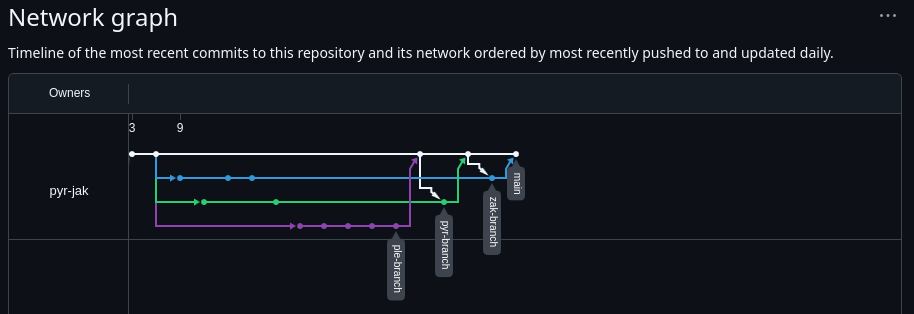
\includegraphics[width=\linewidth,height=0.40\textheight,keepaspectratio]{rys/network_graph.png}%
}{%
  \fbox{\parbox[c][0.20\textheight][c]{0.92\linewidth}{%
    \centering
    \textbf{Miejsce na zrzut ekranu z GitHub Network Graph}\\[4pt]
    \kod{rys/network_graph.png}%
  }}%
}
\caption{Historia gałęzi i punktów scalenia w widoku GitHub Network}
\label{rys:network-graph}
\end{figure}

\clearpage
\section{Analiza problemu}
\label{sec:analiza}

\subsection{Zastosowanie i reprezentacja danych}

Drzewo BST służy do porządkowania danych według klucza.
Porównanie z wartością bieżącego węzła pozwala wybrać jedno
z poddrzew, zamiast sprawdzać wszystkie elementy.
Struktura ta może być wykorzystywana do przechowywania zbiorów
unikatowych wartości i budowy prostych indeksów.

W projekcie węzeł \kod{Node} zawiera wartość \kod{value}
oraz pola \kod{left} i \kod{right}. Pola dzieci są indeksami
w wektorze \kod{tree}; wartość \kod{-1} oznacza brak dziecka.
Indeks korzenia znajduje się w \kod{rootIndex}.
Dla pustego drzewa również wynosi on \kod{-1}.

Rozmieszczenie węzłów w wektorze jest oddzielone od ich połączeń.
Element może leżeć pod dowolnym poprawnym indeksem, o ile pola
dzieci prowadzą do właściwych poddrzew. Sama kolejność wektora
nie musi być posortowana.

\subsection{Sposób działania algorytmu}

Dodawanie rozpoczyna się od korzenia. Wartość mniejsza jest kierowana
do lewego poddrzewa, a większa do prawego. Po dojściu do pustego
połączenia nowy węzeł zostaje dopisany na końcu wektora,
a jego indeks zapisany jako połączenie od rodzica.
Jeżeli wartość już występuje, operacja nie dodaje duplikatu.

Usuwanie rozpoczyna się od wyszukania wartości i zapamiętania
rodzica znalezionego węzła. Gdy wartości nie ma, drzewo pozostaje
bez zmian. Dla znalezionego elementu rozpatrywane są trzy przypadki:
\begin{itemize}
  \item liść zostaje odłączony od rodzica;
  \item węzeł z jednym dzieckiem zostaje zastąpiony połączeniem
        do tego dziecka;
  \item węzeł z dwojgiem dzieci otrzymuje wartość minimum prawego
        poddrzewa, po czym usuwany jest węzeł tego następnika.
\end{itemize}

Usunięcie pozycji wektora przesuwa późniejsze elementy.
Program zmniejsza więc o jeden wszystkie indeksy większe od
usuniętej pozycji, uwzględniając również indeks korzenia.
Metoda \kod{removeTree()} czyści cały wektor i ustawia
\kod{rootIndex} na \kod{-1}. Obiekt może następnie przyjmować
kolejne wartości.

Dla wysokości drzewa $h$ przejście po jednej ścieżce ma koszt $O(h)$.
Dodawanie, wyszukiwanie wartości i wyszukiwanie ścieżki zaczynają się
od korzenia i korzystają z tej reguły. Drzewo nie jest równoważone,
więc przy niekorzystnej kolejności danych
wysokość może rosnąć liniowo z liczbą węzłów $n$.
Skuteczne usunięcie ma koszt $O(n)$ ze względu na przesuwanie
elementów i poprawianie indeksów. Realokacja bufora wektora
może również nadać pojedynczemu dodaniu koszt $O(n)$.

\subsection{Ręczny przykład działania}
\label{sec:przyklad-reczny}

Po dodaniu wartości $1,2,3,8,5$ korzeniem jest 1.
Węzły 2, 3 i 8 tworzą ciąg prawych połączeń, natomiast
5 jest lewym dzieckiem węzła 8.
Rysunek~\ref{rys:przyklad-bst} pokazuje tę strukturę
oraz wynik usunięcia wartości 3. Litery L i P oznaczają
lewe i prawe dziecko.

\begin{figure}[H]
\centering
\begin{tikzpicture}[
  wezel/.style={circle,draw,minimum size=6.5mm,inner sep=1pt,font=\small},
  krawedz/.style={-{Stealth[length=1.6mm]},thin},
  etykieta/.style={font=\scriptsize,fill=white,inner sep=1pt}
]
\node[font=\small\bfseries] at (0.9,0.8) {Przed usunięciem 3};
\node[font=\small\bfseries] at (6.5,0.8) {Po usunięciu 3};

\node[wezel] (a1) at (0,0) {1};
\node[wezel] (a2) at (0.9,-0.9) {2};
\node[wezel] (a3) at (1.8,-1.8) {3};
\node[wezel] (a8) at (2.7,-2.7) {8};
\node[wezel] (a5) at (1.8,-3.6) {5};
\draw[krawedz] (a1) -- node[etykieta,above right] {P} (a2);
\draw[krawedz] (a2) -- node[etykieta,above right] {P} (a3);
\draw[krawedz] (a3) -- node[etykieta,above right] {P} (a8);
\draw[krawedz] (a8) -- node[etykieta,above left] {L} (a5);

\node[wezel] (b1) at (5.6,0) {1};
\node[wezel] (b2) at (6.5,-0.9) {2};
\node[wezel] (b8) at (7.4,-1.8) {8};
\node[wezel] (b5) at (6.5,-2.7) {5};
\draw[krawedz] (b1) -- node[etykieta,above right] {P} (b2);
\draw[krawedz] (b2) -- node[etykieta,above right] {P} (b8);
\draw[krawedz] (b8) -- node[etykieta,above left] {L} (b5);
\end{tikzpicture}

\caption{Drzewo przed usunięciem wartości 3 i po jej usunięciu}
\label{rys:przyklad-bst}
\end{figure}

Węzeł o wartości 3 ma jedno dziecko: węzeł 8.
Program łączy więc rodzica, czyli węzeł 2, bezpośrednio z węzłem 8.
Następnie usuwa pozycję o indeksie 2 z wektora.
Węzły 8 i 5 przesuwają się pod indeksy 2 i 3,
dlatego trzeba poprawić prowadzące do nich połączenia.

Tabela~\ref{tab:zmiana-indeksow} przedstawia zawartość wektora
przed operacją i po korekcie indeksów. Korzeń nadal ma indeks 0.
Kreski w ostatnim wierszu oznaczają pozycję, której po usunięciu
nie ma już w kontenerze.

\begin{table}[H]
\centering
\caption{Zmiana zawartości wektora po usunięciu wartości 3}
\label{tab:zmiana-indeksow}
\small
\begin{tabular}{|c|c|c|c|c|c|c|}
\hline
& \multicolumn{3}{c|}{\textbf{Przed usunięciem}}
& \multicolumn{3}{c|}{\textbf{Po usunięciu}}\\ \hline
\textbf{Indeks} & \textbf{value} & \textbf{left} & \textbf{right}
& \textbf{value} & \textbf{left} & \textbf{right}\\ \hline
0 & 1 & $-1$ & 1 & 1 & $-1$ & 1\\ \hline
1 & 2 & $-1$ & 2 & 2 & $-1$ & 2\\ \hline
2 & 3 & $-1$ & 3 & 8 & 3 & $-1$\\ \hline
3 & 8 & 4 & $-1$ & 5 & $-1$ & $-1$\\ \hline
4 & 5 & $-1$ & $-1$ & --- & --- & ---\\ \hline
\end{tabular}
\end{table}

Po tej operacji metoda \kod{show()} wypisałaby $1,2,8,5$,
zgodnie z kolejnością w wektorze. Opcja inorder w menu podąża
za połączeniami i wypisuje wartości w kolejności $1,2,5,8$.

\subsection{Zależności między modułami a kolejność scalania}
\label{sec:kolejnosc-scalania}

Jeżeli obie gałęzie robocze wprowadzają zależne zmiany, najpierw
należy scalić do \kod{main} operacje drzewa. Na przykład zapis
binarny używa metody \kod{preorderValues()}, a menu korzysta
z \kod{findPath()}. Zmiany w deklaracjach tych metod powinny
trafić do gałęzi z interfejsem, zanim jej PR zostanie scalony.
W tym celu włącza się do niej aktualny stan \kod{main}
zgodnie z procedurą z punktu~\ref{sec:konflikt-scalania}.

Po aktualizacji gałęzi interfejsu sprawdza się kompilację programu
i uruchamia próby zależnych operacji. Dla \kod{findPath()} można
porównać ścieżkę do znanego węzła, a dla zapisu binarnego
zapisać drzewo, opróżnić je i odtworzyć z pliku. Wyniki
tych prób można dołączyć do PR-a jako podstawę przeglądu.

\clearpage
\section{Projektowanie}

\subsection{Podział odpowiedzialności}

Program składa się z interfejsu konsolowego, klasy reprezentującej
drzewo oraz modułu operacji plikowych. Tabela~\ref{tab:moduly}
pokazuje, za co odpowiada każda część. Deklaracje struktur i metod
umieszczono w plikach nagłówkowych. Ich szczegółowy wykaz zawiera
również dokumentacja wygenerowana przez Doxygen~\cite{doxygen-bst}.

\begin{tabela}{Podział programu na moduły}
              {Podział programu na moduły}
              {\label{tab:moduly}}
\small
\begin{tabularx}{\linewidth}{|L{4.2cm}|Y|}
\hline
\textbf{Pliki} & \textbf{Odpowiedzialność}\\ \hline
\kod{main.cpp} & Wyświetla menu, sprawdza dane wejściowe i przekazuje
                 operacje do \kod{BST} lub \kod{BSTFile}.\\ \hline
\kod{BST.h}, \kod{BST.cpp} & Definiują węzeł \kod{Node} i klasę
  \kod{BST}. Zarządzają węzłami, wyszukiwaniem, przejściami,
  rysunkiem drzewa i jego zapisem tekstowym.\\ \hline
\kod{BSTFile.h}, \kod{BSTFile.cpp} & Zawierają metody statyczne
  do zapisu i odczytu binarnego oraz do importu tekstowego.
  Korzystają z metod publicznych klasy \kod{BST}.\\ \hline
\kod{CMakeLists.txt} & Definiuje budowanie programu
  \kod{Drzewo_BST} z trzech plików \kod{.cpp}.\\ \hline
\end{tabularx}
\end{tabela}

\subsection{Warunki poprawności drzewa}

Wektor \kod{tree} zawiera wszystkie węzły należące do drzewa.
W drzewie niepustym \kod{rootIndex} wskazuje prawidłową pozycję
w wektorze. Każdy pozostały węzeł jest osiągalny z korzenia przez
jedno połączenie od rodzica. Pola dzieci przyjmują wartość $-1$
albo indeks istniejącego węzła. Przez całą ścieżkę obowiązuje
porządek BST opisany w rozdziale~\ref{sec:analiza}.

Indeks jest szczegółem reprezentacji i może zmienić się po
usunięciu pozycji z wektora. Z tego powodu metody publiczne
przyjmują klucze typu \kod{int}, a \kod{findPath()} i
\kod{preorderValues()} zwracają wartości węzłów. Program główny
może więc używać tych metod bez dostępu do wektora i indeksów.

\Needspace{11\baselineskip}
\subsection{Menu konsolowe}
\label{sec:menu}

Opcje menu zestawiono w tabeli~\ref{tab:menu}. W trybach dodawania
i usuwania można podać wiele wartości rozdzielonych białymi znakami.
Wpisanie małej litery \kod{q} przywraca menu. Wyszukiwanie ścieżki
przyjmuje jedną wartość i po wyświetleniu wyniku wraca do menu.

\begin{tabela}{Opcje menu programu}{Opcje menu programu}{\label{tab:menu}}
\small
\begin{tabularx}{\linewidth}{|c|Y|L{5.1cm}|}
\hline
\textbf{Opcja} & \textbf{Działanie} & \textbf{Metoda}\\ \hline
1 & Dodawanie elementów & \kod{BST::addNode()}\\ \hline
2 & Usuwanie elementów & \kod{BST::removeNode()}\\ \hline
3 & Usuwanie całego drzewa & \kod{BST::removeTree()}\\ \hline
4, 5, 6 & Przejścia preorder, inorder i postorder.
Każda opcja wypisuje również rysunek drzewa. &
\kod{preorder()}, \kod{inorder()}, \kod{postorder()}, \kod{printTree()}\\ \hline
7 & Wyszukanie ścieżki od korzenia & \kod{BST::findPath()}\\ \hline
8 & Zapis do \kod{drzewo.txt} & \kod{BST::saveToTextFile()}\\ \hline
9 & Zapis do \kod{drzewo.bin} & \kod{BSTFile::saveBinary()}\\ \hline
10 & Odtworzenie drzewa z \kod{drzewo.bin} & \kod{BSTFile::loadBinary()}\\ \hline
11 & Dodanie liczb ze wskazanego pliku tekstowego & \kod{BSTFile::loadText()}\\ \hline
12 & Zakończenie programu & Powrót z \kod{main()}\\ \hline
\end{tabularx}
\end{tabela}

Numery opcji i wartości są odczytywane jako pojedyncze tokeny.
Program sprawdza, czy cały token można odczytać jako liczbę typu
\kod{int}. Wpisy takie jak \kod{3x}, \kod{3.5} i liczby spoza
zakresu typu są odrzucane. Liczba całkowita spoza zakresu opcji
1--12 powoduje ponowne wyświetlenie menu z komunikatem o błędnej
opcji. Zakończenie strumienia wejściowego kończy pracę programu.

\Needspace{9\baselineskip}
\subsection{Dane zapisywane w plikach}
\label{sec:formaty}

Zapis tekstowy tworzy plik \kod{drzewo.txt} z jedną liczbą w każdym
wierszu. Zapis binarny tworzy plik \kod{drzewo.bin}, który zaczyna się
od licznika typu \kod{std::uint64_t}, po którym występują kolejne
wartości typu \kod{int}. W obu przypadkach wartości są pobierane
w kolejności preorder. Plik binarny zapisany przez program zawiera
więc $8 + n \cdot \texttt{sizeof(int)}$ bajtów dla $n$ węzłów.
Program zapisuje typy w ich reprezentacji maszynowej. Przy wymianie
plików między platformami wymagane są zgodne rozmiary i kolejność
bajtów zapisywanych typów.

Wstawianie wartości w kolejności preorder do pustego drzewa
odtwarza jego kształt. Pierwsza wartość staje się korzeniem.
Przed wartościami każdego poddrzewa występuje jego własny korzeń,
więc ta sama zasada działa na kolejnych poziomach. Węzły w wektorze
mogą po odczycie mieć inne indeksy, ponieważ wynikowy wektor jest
budowany w kolejności wstawiania.

Odczyt binarny zastępuje bieżące drzewo wynikiem po sprawdzeniu
całego pliku. Import tekstowy dopisuje unikatowe liczby do
bieżącego drzewa. W opcji~11 należy podać ścieżkę w jednym
wierszu. Ścieżka może zawierać spacje i jest podawana bez
cudzysłowów. Ścieżki względne są rozwiązywane względem katalogu
roboczego programu. Jeśli celem jest odtworzenie drzewa z pliku
\kod{drzewo.txt}, należy najpierw je opróżnić opcją~3.

\clearpage
\section{Implementacja}

\subsection{Dodawanie i usuwanie węzłów}

Metoda \kod{addNode()} zapamiętuje rozmiar wektora i wywołuje
rekurencyjną metodę \kod{insert()}. Wzrost rozmiaru oznacza
dodanie nowego węzła i wynik \kod{true}. Wartość już obecna
w drzewie kończy operację wynikiem \kod{false}. Po powrocie
z wywołania rekurencyjnego rodzic jest ponownie odczytywany
przez indeks. Dzięki temu dodanie elementu pozostaje poprawne
także po przeniesieniu bufora wektora. Pokazuje to
listing~\ref{lst:wstawianie}.

\listingpliku[firstline=25,lastline=34,firstnumber=25,
  caption={Aktualizacja połączenia po wstawieniu do poddrzewa},
  label={lst:wstawianie}]{kod/BST.cpp}

Metoda \kod{removeNode()} wyszukuje iteracyjnie wartość i zapamiętuje
indeks rodzica. W przypadku dwojga dzieci szuka następnika, schodząc
najpierw w prawo, a następnie maksymalnie w lewo. Kopiuje jego
wartość do usuwanego węzła, a fizycznie usuwa następnika. Następnik
może mieć prawe dziecko, które przejmuje jego dotychczasowe miejsce.
W przypadku usuwania korzenia z najwyżej jednym dzieckiem
aktualizowane jest bezpośrednio pole \kod{rootIndex}.

Metoda usuwa pozycję z wektora dopiero po przełączeniu połączeń.
Potem zmniejsza wszystkie indeksy większe od usuniętej pozycji.
Zwraca \kod{true} po usunięciu węzła i \kod{false}, jeśli klucza
nie znaleziono. Metoda \kod{removeTree()} wywołuje \kod{tree.clear()}
i ustawia \kod{rootIndex} na $-1$. Wektor zachowuje pojemność do
ponownego wykorzystania.

\Needspace{7\baselineskip}
\subsection{Wyszukiwanie, przejścia i rysunek}

Metoda \kod{findElement()} zwraca informację o obecności klucza.
Używana przez menu metoda \kod{findPath()} dodatkowo zapisuje
wartości napotkanych węzłów. Znaleziona ścieżka obejmuje korzeń
i szukany węzeł. Gdy wyszukiwanie dojdzie do indeksu $-1$,
metoda zwraca pusty wektor. Jeżeli szukanym kluczem jest korzeń,
wynik zawiera jedną wartość.

\kod{preorderValues()} używa wektora indeksów jako stosu.
Pobiera węzeł, dopisuje jego wartość do wyniku, a następnie
odkłada na stos najpierw prawe, potem lewe dziecko. Dzięki
temu lewe poddrzewo jest odwiedzane wcześniej. Z wyniku tej
metody korzystają przejście preorder i oba tryby zapisu.
Inorder odwiedza lewe poddrzewo, węzeł i prawe poddrzewo,
uzyskując wartości rosnąco. Postorder wypisuje węzeł po obu
poddrzewach. Te dwa przejścia są rekurencyjne. Metoda
\kod{show()} jest osobną funkcją klasy i odczytuje wartości
w fizycznej kolejności wektora.

\kod{printTree()} wywołuje rekurencyjną metodę \kod{drawBranch()},
która tworzy etykiety z wartości liczbowych, przydziela im
miejsce w kolejności inorder i buduje wiersze rysunku. Między
poziomami drzewa umieszcza wiersze z łącznikami. Dla węzła
z dwojgiem dzieci pozycja środka etykiety jest wyznaczana
na podstawie pozycji obu dzieci. Dla pustego drzewa
\kod{printTree()} wypisuje komunikat \kod{Drzewo jest puste.}

\subsection{Sprawdzanie danych podczas odczytu}

\kod{loadBinary()} zaczyna od odczytania licznika, a następnie
wstawia kolejne wartości do nowego obiektu \kod{BST}. Wykrywa
brak wymaganych danych, duplikaty i nadmiarowe bajty.
Dopiero po sprawdzeniu końca pliku przenosi wynik do drzewa
używanego w menu. Poprawny zapis pustego drzewa zawiera
sam licznik o wartości zero. Wczytanie takiego pliku
opróżnia bieżące drzewo.

\kod{loadText()} zaczyna od kopii istniejącego drzewa. Czyta
tokeny oddzielone białymi znakami i sprawdza, czy każdy mieści
się w zakresie \kod{int} i składa się w całości z zapisu
liczby całkowitej. Duplikaty są pomijane przez \kod{addNode()}.
Pusty plik tekstowy zostaje odczytany poprawnie i nie dodaje
żadnych wartości. Przy błędzie odczytu albo błędnym tokenie
bieżące drzewo zachowuje swój stan także wtedy, gdy wcześniej
przetworzono już część pliku. Metody zapisu zwracają błąd
przy problemie z otwarciem, zapisem lub zamknięciem pliku.
Oba zapisy otwierają plik w trybie nadpisywania, więc błąd po
otwarciu może pozostawić plik częściowy.

\Needspace{12\baselineskip}
\subsection{Sprawdzenie działania}
\label{sec:testy}

Kod skompilowano w trybie C++14. Do pustego drzewa wprowadzono
kolejno liczby 8, 3, 10, 1, 6, 14, 4, 7 i 13. Listing~\ref{lst:przejscia}
zawiera wiersze z wynikami trzech przejść odczytane z konsoli.

\begin{lstlisting}[style=terminal,caption={Wyniki trzech przejść drzewa},label={lst:przejscia}]
Preorder: 8 3 1 6 4 7 10 14 13
Inorder: 1 3 4 6 7 8 10 13 14
Postorder: 1 4 7 6 3 13 14 10 8
\end{lstlisting}

Tabela~\ref{tab:proby} zestawia pozostałe próby wykonane z menu.
Próby importu wykonano z drzewa złożonego z węzła o wartości 8.

\begin{tabela}{Próby wykonane w menu}{Próby wykonane w menu}
              {\label{tab:proby}}
\small
\begin{tabularx}{\linewidth}{|L{4.8cm}|Y|}
\hline
\textbf{Próba} & \textbf{Zaobserwowany wynik}\\ \hline
Ponowne dodanie liczby 6 & Program zgłosił duplikat.\\ \hline
Wyszukanie 7 i 42 & Ścieżka do 7 to $8\to3\to6\to7$.
Program zgłosił brak 42.\\ \hline
Usunięcie korzenia 8 & Następnikiem został 10. Przejście inorder dało
$1,3,4,6,7,10,13,14$.\\ \hline
Zapis tekstowy i binarny & Plik tekstowy zawierał dziewięć wartości
w kolejności preorder. Odczyt zapisu binarnego po opróżnieniu drzewa
przywrócił ten sam wynik preorder i ten sam rysunek.\\ \hline
Odczyt obciętego pliku binarnego & Program zgłosił błąd,
a drzewo zachowało dotychczasową zawartość.\\ \hline
Import tekstu \kod{-4 8 9} &
Przejście inorder dało $-4,8,9$. Powtórzona wartość 8 wystąpiła raz.\\ \hline
Import tekstu \kod{-4 9x} &
Program zgłosił błąd. Drzewo nadal zawierało tylko wartość 8.\\ \hline
\end{tabularx}
\end{tabela}

\clearpage
\section{Wnioski}

Indeksowa reprezentacja drzewa pozwoliła przechowywać węzły
w jednym wektorze i oddzielić ich rozmieszczenie od logicznych
połączeń. Konsekwencją tego wyboru jest aktualizacja indeksów
po usunięciu pozycji. Nawet gdy węzeł można znaleźć szybko,
udane usunięcie wymaga przejścia po pozostałych elementach
wektora i ma koszt $O(n)$.

Wyszukiwanie wartości i ścieżki oraz porównania podczas
wstawiania zależą od wysokości drzewa $h$. Kolejność danych
ma więc znaczenie. Jeżeli liczby są podawane rosnąco, każdy
następny węzeł staje się prawym dzieckiem poprzedniego.
Wówczas $h$ rośnie liniowo, a budowanie drzewa przez kolejne
wstawienia może wymagać $O(n^2)$ czasu. Dotyczy to również
odtwarzania takiego drzewa z pliku binarnego. Rekurencyjne
wstawianie, inorder, postorder i rysowanie korzystają
ze stosu wywołań o głębokości rzędu $h$.

Każde z trzech przejść odwiedza wszystkie węzły i ma koszt
czasowy $O(n)$, bez uwzględnienia rysunku konsolowego.
Implementacja preorder gromadzi cały wynik w wektorze
i wykorzystuje na ten cel $O(n)$ dodatkowej pamięci.

Próby z podrozdziału~\ref{sec:testy} pokazują, że kolejność
przejścia można dobrać do celu. Inorder daje uporządkowaną
listę kluczy, a preorder wystarcza do zapisania i odtworzenia
kształtu drzewa bez przechowywania indeksów. W obu trybach
odczytu wynik trafia do bieżącego drzewa po sprawdzeniu
danych. Dzięki temu błędny plik nie pozostawia częściowo
wczytanego drzewa.

Naturalnym rozszerzeniem przy wymianie danych między różnymi
platformami byłby format binarny z określoną kolejnością
bajtów i stałą szerokością klucza. Przy pracy z dużymi,
uporządkowanymi zbiorami danych istotnym kierunkiem rozwoju
byłoby ograniczenie wysokości drzewa i głębokości rekurencji.


\newpage
\clearpage
\phantomsection
\addcontentsline{toc}{section}{Literatura}
\begingroup
\raggedright
\bibliographystyle{unsrt}
\bibliography{bibliografia}
\endgroup

\newpage
\medskip
\phantomsection
\addcontentsline{toc}{section}{Spis rysunków}
\listoffigures

\newpage
\medskip
\phantomsection
\addcontentsline{toc}{section}{Spis tabel}
\listoftables

\newpage
\medskip
\phantomsection
\addcontentsline{toc}{section}{Spis listingów}
\lstlistoflistings
\end{document}
